%%%%%%%%%%%%%%%%%%%%%%%%%%%%%%%%%%%%%
%                                   %
% Compile with XeLaTeX and biber    %
%                                   %
% Questions or comments:            %
%                                   %
% joshua dot mcneill at uga dot edu %
%                                   %
%%%%%%%%%%%%%%%%%%%%%%%%%%%%%%%%%%%%%

\documentclass{beamer}
  % Read in standard preamble (cosmetic stuff)
  %%%%%%%%%%%%%%%%%%%%%%%%%%%%%%%%%%%%%%%%%%%%%%%%%%%%%%%%%%%%%%%%
% This is a standard preamble used in for all slide documents. %
% It basically contains cosmetic settings.                     %
%                                                              %
% Joshua McNeill                                               %
% joshua dot mcneill at uga dot edu                            %
%%%%%%%%%%%%%%%%%%%%%%%%%%%%%%%%%%%%%%%%%%%%%%%%%%%%%%%%%%%%%%%%

% Beamer settings
% \usetheme{Berkeley}
\usetheme{CambridgeUS}
% \usecolortheme{dove}
% \usecolortheme{rose}
\usecolortheme{seagull}
\usefonttheme{professionalfonts}
\usefonttheme{serif}
\setbeamertemplate{bibliography item}{}

% Packages and settings
\usepackage{fontspec}
  \setmainfont{Charis SIL}
\usepackage{hyperref}
  \hypersetup{colorlinks=true,
              allcolors=blue}
\usepackage{graphicx}
  \graphicspath{{../../figures/}}
\usepackage[normalem]{ulem}
\usepackage{enumerate}

% Document information
\author{M. McNeill}
\title[FREN2001]{Français 2001}
\institute{\url{joshua.mcneill@uga.edu}}
\date{}

%% Custom commands
% Lexical items
\newcommand{\lexi}[1]{\textit{#1}}
% Gloss
\newcommand{\gloss}[1]{`#1'}
\newcommand{\tinygloss}[1]{{\tiny`#1'}}
% Orthographic representations
\newcommand{\orth}[1]{$\langle$#1$\rangle$}
% Utterances (pragmatics)
\newcommand{\uttr}[1]{`#1'}
% Sentences (pragmatics)
\newcommand{\sent}[1]{\textit{#1}}
% Base dir for definitions
\newcommand{\defs}{../definitions}


  % Packages and settings

  % Document information
  \subtitle[Nos loisirs (encore)]{Nos loisirs (encore)}

\begin{document}
  % Read in the standard intro slides (title page and table of contents)
  \begin{frame}
    \titlepage
    \tiny{Office: % Basically a variable for office hours location
Gilbert 121\\
          Office hours: % Basically a variable for office hours
 lundi, mercredi, vendredi 10:10--11:10
}
  \end{frame}

  \begin{frame}{Annonces}
    \begin{itemize}
      \item Le devoir 2 à rendre le 23 septembre.
      \item[] \tinygloss{Homework 2 to be turned in September 23rd.}
    \end{itemize}
  \end{frame}

  \begin{frame}{Révision}
    \begin{center}
      \begin{tabular}{l | l l | l l}
  \multicolumn{5}{c}{faire \gloss{to do}} \\
      & \multicolumn{2}{l |}{singulier} & \multicolumn{2}{l}{pluriel} \\
  \hline
  1re & je         & fais               & nous        & faisons \\
  2e  & tu         & fais               & vous        & faites \\
  \hline
  3e  & il (masc)  &                    & ils (masc)  & \\
      & elle (fem) & fait               & elles (fem) & font \\
      & on         &                    &             & \\
\end{tabular}

    \end{center}
  \end{frame}

  \begin{frame}{}
    \begin{center}
      \Large Quiz
    \end{center}
  \end{frame}

  \begin{frame}{Un sondage}
    \begin{columns}
      \column{0.5\textwidth}
        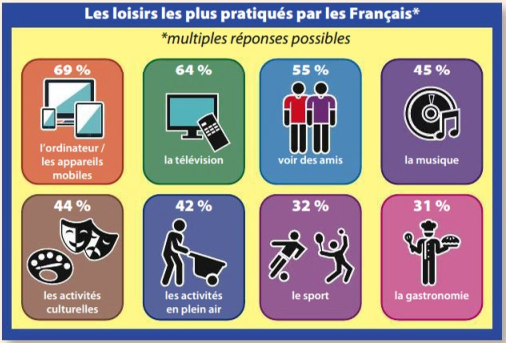
\includegraphics[scale=0.75]{loisirs_france.png} \\
        Les Français...
        \begin{itemize}
          \item travaillent 35 heures par semaine.
          \item prennent 5 semaines de vacances au moins.
        \end{itemize}
      \column{0.5\textwidth}
        Comparons les loisirs des Français avec les loisirs de la classe. \\
        \tinygloss{Let's compare the leisure activities of the French with the leisure activities of the class.}
        \begin{enumerate}
          \item Demandez $\to$ \emph{Qui fait de la musique?}
          \item Comptez les mains
          \item Annoncez les résultats $\to$ \emph{6 étudiants font de la musique. C'est 30 pour cent.}
        \end{enumerate}
    \end{columns}
  \end{frame}

  \begin{frame}{}
    \begin{center}
      \Large Questions?
    \end{center}
  \end{frame}
\end{document}
